
\documentclass[a4paper]{article}

\usepackage{INTERSPEECH_v2}

\title{Predicting age using synchronized MEG and speech recordings of children}
\name{Demetres Kostas$^1$, Elizabeth W. Pang$^2$, Frank Rudzicz$^{3,1,*}$}
\address{
  $^1$University of Toronto; $^2$SickKids Research Institute;\\
  $^3$Toronto Rehabilitation Institute-UHN; Toronto Canada}
\email{$^*$frank@cs.toronto.edu}

\usepackage{soul,color} 
\newcommand{\FR}[1]{{\small \textcolor{red}{\hl{#1}}}}
\newcommand{\DK}[1]{{\small \textcolor{blue}{\hl{#1}}}}

\begin{document}

\maketitle
% 
\begin{abstract}
% FR:
Evidence suggests that there is a correlation between the synchronization of different brain areas and the development of language in children. In order to explore this correlation, we attempt to predict the age of children (4-18 years old) using synchronized magneto-encephalographic (MEG) and audio recordings of verb generation and syllable production tasks. We extract time-windowed features from both MEG and audio recordings to capture time and frequency domain signal characteristics, then investigate the correlations between audio and brain recording features. We also use regularized linear regression to predict the age of subjects using audio, MEG and MEG+audio feature sets, and obtain consistent RMSE.
\end{abstract}


\noindent\textbf{Index Terms}: Brain-computer interfaces, speech production, child language acquisition

\section{Introduction}

The synchronization of neural oscillations between distributed brain regions has been an effective mechanistic explanation for various cognitive and perceptual processes \cite{Fries2015,Nakasaki1989,NeuralSync}. \FR{Yes -- 1 more sentence about brain synchronization and processing. A broad definition. DK-TODO}. For example, Doesburg {\em et al.} \cite{Doesburg2016} observed an increased synchrony with the increase of age during verb-generation (VG) tasks in children and adolescents, and observed a significant increase in the number of synchronous regions with older adolescents, compared with younger children. Furthermore, Yu {\em et al.} \cite{Yu2014} noticed distinct profiles of de-synchrony in VG tasks for children within five age ranges (i.e., 4-6, 7-9, 10-12, 13-15, and 16-18 years of age). These findings indicate the possibility of inferring a child's age from observed MEG data, provided the ability to convey synchronicity and coordinated activity. The extraction of common spectral features such as the fast Fourier transform (FFT) magnitude and features like signal energy have shown some success with various classifiers in accurately differentiating different persons from electroencephalographic (EEG) experiments \cite{Nguyen2012, Poulos2001}.

Previous work with MEG includes detecting hand movement \cite{Asano2009}, identifying schizophrenia \cite{Ince2008}, and on discriminating between sets of imagined words \cite{Guimaraes2007}. To classify between three different hand movements\footnote{Corresponding to the signs in the game of `rock, paper, scissors'.}, Asano {\em et al.} \cite{Asano2009} used an adaptive spatial filter, principal components analysis (PCA) and a support vector machine (SVM) to achieve 62.6\% on held-out test data. In Ince {\em et al.} \cite{Ince2008}, a subject performed a working memory functional task while MEG data were recorded; an SVM with recursive feature elimination (SVM-RFE) was then used to both select a concise feature set and to identify schizophrenia. SVM-RFE recursively discarded features that did not significantly contribute to the margin of the SVM classifier to prevent excessive overfitting on the training set, and achieved 83.8\% to 91.9\% on the test data.

Closer to our work, Guimaraes {\em et al.} \cite{Guimaraes2007} classified sets of 7-9 imagined words in two subtasks. In the first, the subject was simply required to attentively listen to a spoken word, while in the second the subject was shown each word visually and told to recite it
silently. Those data were then examined using linear discriminant classification and SVM algorithms to classify each
channel, and further analyzed in terms of the effects of spatial PCA, independent components analysis (ICA) and second-order
blind identification decomposition. By combining channels, Guimaraes {\em et al.} achieved 60.1\% mean classification
rate on nine auditory words and 97.5\% maximum mean classification rate on two-word problems.


We hypothesized that the accuracy of a regression model trained using a combined dataset of MEG and audio features would be greater than that of models trained with only audio and MEG respectively. We postulated that this would be due to the fact that MEG data would represent information about synchronicity and activity localization that would not otherwise be apparent with speech alone.

\section{Data}

These data were originally recorded for work on age- and sex-related developmental language differences by Doesburg \emph{et al.} and Yu \emph{et al.} \cite{Doesburg2016, Yu2014}. Table \ref{tab:subjects} summarizes some participant demographics. Each participant spoke English as their first language and had no known or suspected histories of speech, language, hearing, or developmental disorders, according to their parents. Prior to the experiment, children received two standardized clinical tests: the Peabody Picture Vocabulary Test (PPVT) \cite{Dunn97} and the Expressive Vocabulary Test (EVT) \cite{EVT}. All children's scores were at or above expected scores for their ages on the PPVT and EVT, and their speech showed no signs of articulatory difficulties. In total, 80 participants were right-handed, 5 were left-handed, and 7 were ambidextrous; there is no significant variation of handedness with age.

Three distinct speech-elicitation stimuli were used. The first two were of the monosyllable /{\em pah}/ and the multisyllabic sequence /{\em pah tah kah}/, respectively. These were simple enough for young children and are part of the diadochokinetic rate (DDK) test, which can be used to evaluate neuromuscular control in motor speech disorders. The incisive nature of these stimuli for measuring speech production make them ideal for this study. Prior to acquisition, the experimenter demonstrated the productions of each stimuli, without word-like prosodic patterns. The third experiment was an overt verb generation (VG) task in English, where subjects are presented with an image they are familiar with, and are asked to produce a verb associated with the object \cite{Doesburg2016}.

Recordings were made in a sound-proof room, with each participant lying supine in a magnetically shielded room in the Neuromagnetic Lab of the Hospital for Sick Children in Toronto, using a CTF whole-head MEG system (MEG International Services Ltd., Coquitlam, BC, Canada). The system recorded all 151 MEG channels, and a single audio channel, with a sampling rate of 4 kHz. % DK The following was done as part of processing steps: The MEG signals were resampled at 200Hz, and band pass filtered between 0.5Hz and 100 Hz.

\section{Methods}

%Overview of experiments, data processing and analysis performed

\subsection{Data processing}

\begin{table}[t]
  \caption{Participant demographics, across stimuli type. The two tasks involve considerable participant overlap.}
  \label{tab:subjects}
  \centering
  \begin{tabular}{ c@{}c c c c }
    \toprule
    \multicolumn{1}{c}{\textbf{Stimuli}} & \multicolumn{1}{c}{\textbf{Age}} & \multicolumn{1}{c}{\textbf{Subjects}} & \multicolumn{1}{c}{\textbf{Trials}}  & \multicolumn{1}{c}{\textbf{M/F Split}} \\
    \midrule
    /{\em pah}/~~~                    & $4.1-18.4$   &   $92$   &   $115$   &   $-$ \\
    /{\em pah tah kah}/~~~                & $4.1-18.4$   &   $89$   &   $115$   &   $-$ \\
    VG~~~                      & $-$   &   $31$   &   $81$    &   $-$  \\
    \bottomrule
  \end{tabular}
\end{table}

We resample MEG signals at 200 Hz, and band-pass filter between 0.5 Hz and 100 Hz, to remove offsets and accommodate the canonical ranges of delta, theta, alpha, beta, and gamma activity. We remove electro-ocular (EOG) artifacts using automated blind source separation (BSS), and measure  signal complexities using fractal dimensions. Auto-BSS filters EOG artifacts using the SOBI algorithm in AAR's implementation.

We then apply info-max independent component analysis (ICA) \cite{Bell1995} to determine statistically independent sub-components of the MEG recordings, across all subjects. This was done by appending MEG recordings for all subjects into a single 151-channel matrix for each of the 4 tests \FR{which are?} performed using the EEGLAB toolbox \cite{Delorme04eeglab}. We then apply the resulting sphering and weight matrices, determined by ICA for each test condition, to each subject's respective recordings. These recordings (i.e., both MEG and audio separately) are then separated into windowed epochs corresponding to $-500$ ms to $+1500$ ms frames around the onset of the stimuli prompt.

\subsection{Feature extraction}

We extract a total of 156 acoustic features and 4681 MEG features from each epoch using openSMILE \cite{Eyben13-RDI}. These are calculated using 50 ms rectangular windows, with a 25 ms overlap of the previous window for each successive window, resulting in a total of 79 windows per datapoint.

\subsubsection{Audio features}

Features to represent spectral activity are calculated, for each window, using both a 128-point fast Fourier transform and linear predictive coding coefficients. Additionally, the statistical moments, mean (also absolute mean, quadratic mean, and aforementioned means calculated using only non-zero values), variance, skewness. and kurtosis are calculated. Finally, the root-mean-squared and log of the signal energy are also calculated for each window.

\subsubsection{MEG features}

We extract 31 features for each of the 151 independent components derived from the MEG data. These consist of an 8-point fast Fourier transform, statistical moments, and energy calculation identical to the audio signal, and the autocorrelation function (ACF) calculated using the fast Fourier transform (FFT) and its inverse (iFFT) for window $w$:

\begin{equation}
  ACF(w) = iFFT(|FFT(w)|^2)
  \label{eq1}
\end{equation}

\subsection{Data analysis}

First, we identify correlations among extracted features, in order to demonstrate evidence for predictive potential. We then train regularized multilinear regression models to predict a subject's age.

\subsubsection{Correlation}

We used standard Pearson correlation between MEG and audio features, for each experiment set separately. We set significance for $p$-values at $\alpha = 10^{-4}$ and the coefficient $r$'s absolute value $\text{abs}(r) > 0.2$.  Furthermore, we compute correlation of MEG and audio features, with respect to age, over the entire data set, to identify features with a potentially stronger predictive capability for regression.

\subsubsection{Multilinear regression}

We train multilinear regression models to predict age using each of the \textit{Audio}, \textit{MEG}, and the fused \textit{Audio+MEG} datasets respectively. We use 10-fold cross-validation within each dataset. The test and training sets are selected to have a similar mean and standard deviation over the ages of participants. We perform Bayesian parameter optimization using Hyperopt \cite{Bergstra2013} on the first fold of data to determine an appropriate learning rate and regularization factor for all training. % FR I'll need this to be clarified to me, at some point.

Since the number of features multiplied by the number of time windows exceeds the total number of data points available to train, we reduce the dimensionality of the MEG data (i.e., {\em MEG-red}) by selecting only those features from that set that have significant correlations, as defined above.

\section{Results}

\subsection{Correlations}

\subsubsection{MEG vs. audio: /pah/}

Only $0.0163$\% of the $156 \times 4681$ correlations for this experiment set are significant, on these data. Therefore, there appears to be little redundancy between the \textit{selected} MEG and audio features \FR{Is this true?? You select features that are specifically a closely related as possible...}. Of these significant correlations, all were with respect to three audio features. These features corresponded to sequential FFT bins that represent the frequency range (340 - 400)Hz. The most correlated MEG feature is the autocorrelation measure for six different components.

\subsubsection{MEG vs. audio: /pah tah kah/}

Under this test condition, $0.0116$\% of correlations between features are significant and, similar to the /{\em pah}/ experiment, these correlations heavily involve the audio features that represent frequencies 320-400 Hz, in addition to some features that represent much lower frequencies 80-160 Hz, which may be due to noise in the environment. Also similar to the /{\em pah}/ experiment, the autocorrelation feature seems to be significantly correlated for 8 components, three of which are the same components as the /{\em pah}/ experiment.

% The frequency range 340-400 pops up both times, it seems to be too low to be related to formats or F0, but I can't say for sure because for some reason I commented out the formants section of my opensmile configuration, I calculate the LPC anyway, but I didn't even leave myself a note as to why I did that...

\subsubsection{MEG vs. audio: Verb Generation}

\begin{figure}[t]
  \centering
  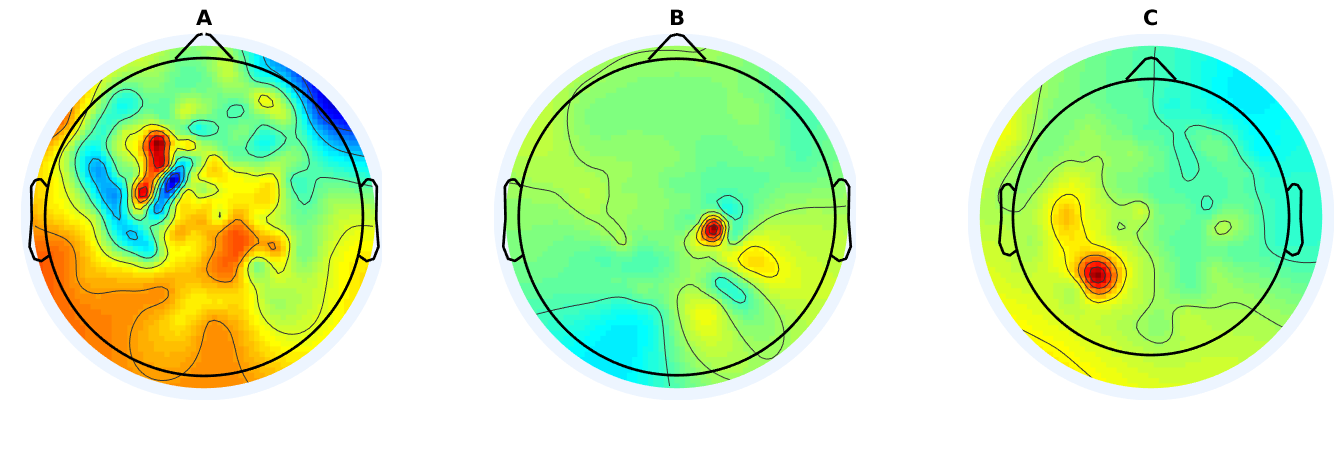
\includegraphics[width=\linewidth]{AllComponents.png}
  \caption{Graphical illustrations (using \cite{Delorme04eeglab}) of the independent components with features most correlated with audio features, from left to right, /{\em pah}/, /{\em pah tah kah}/ and verb generation tasks. \FR{provide some context in the text}}
  \label{fig:components}
\end{figure}

\subsubsection{All features vs. age}

The 172 selected features here are all MEG features. This set includes the autocorrelation features of eight components -- including the first (highest entropy) component -- in addition to the entire available frequency spectrum of four of these \FR{ICA?} components and one other. The fact that spectral features are relatively strongly correlated with age might provide evidence that synchronization may be distinguishing factor across age, but additional feature analysis will be necessary to confirm this. 

The correlation of the 99\textsuperscript{th} \DK{(note to say 99th (low) greatest entropy?)} \FR{??} computed component has correlation coefficients $\text{abs}(r)>0.3$ for nearly all of its features, which was true of no other components considered. Examining the physical representation of these components with respect to each of the three experiments, there were no discernible similarities to note. Three other components also had features with correlation $\text{abs}(r)>0.3$, for features that corresponded to various mean variants.

\subsection{Regression}

The regression performance across the 10 folds seems to suggest that a multilinear regression model trained using both audio and the reduced (i.e., highly correlated) MEG feature sets performs better than either Audio or MEG feature sets alone. Without  reducing the MEG feature set, regression performance is no better than that for Audio alone. Models trained using some MEG features also  perform more consistently (i.e., with lower variance) than with Audio features exclusively.

When trained using the highly correlated MEG features, regression performance is nearly equivalent to its exhaustive counterpart. There is a fairly marked reduction in variance, but performance does not increase until Audio and MEG features are combined. This may be surprising, considering that the MEG features are relatively correlated with age. This could suggest somewhat complementary information between data sets. % FR: in future, a measure of mutual information should be computed.

\begin{table}[t]
  \caption{Root mean squared error (RMSE) in years, of ten-fold cross validation for each of the datasets. Audio features combined with reduced MEG features show the best prediction capability.}
  \label{tab:rmse}
  \centering
  \begin{tabular}{ l@{}c  c }
    \toprule
    \multicolumn{1}{c}{\textbf{Dataset}} & \multicolumn{1}{c}{\textbf{Mean}} & \multicolumn{1}{c}{\textbf{Variance}} \\
    \midrule
    Audio~~~                             & ~~~$4.103$         &     $0.473$~~~       \\
    MEG~~~                               & ~~~$4.896$         &     $0.234$~~~       \\
    Audio+MEG~~~                         & ~~~$4.109$         &     $0.244$~~~       \\

    MEG (red.)~~~                        & ~~~$5.081$         &     $0.142$~~~       \\
    Audio+MEG (red.)~~~                  & ~~~$3.370$         &     $0.248$~~~       \\
    \bottomrule
  \end{tabular}
\end{table}

\section{Discussion}

\begin{itemize}
\item ICA components are different for each experiment type, but we treat them to some degree as if they were the same ie. weight for feature 1 could be from any of the experiments
\item 340-400Hz Frequency consistently correlated with MEG features, would expect this to be average F0 or /ah/ formant, but too low, did I calculate wrong? 1/50ms => 20Hz FFT buckets. Could say formants are missing, and would be a good feature to have if done again.
\item does some of the regression results section belong here?
\end{itemize}

Frank wants to write section outlining caveats

We show a mild confirmation of our hypothesis.

\section{Acknowledgements}

We thank Rui Janson for his help performing automated EOG removal.


\bibliographystyle{IEEEtran/bibtex/IEEEtran}

\bibliography{IS2017}


\end{document}
